\section{Arquitectura de la Solución}

\begin{figure}[H]
    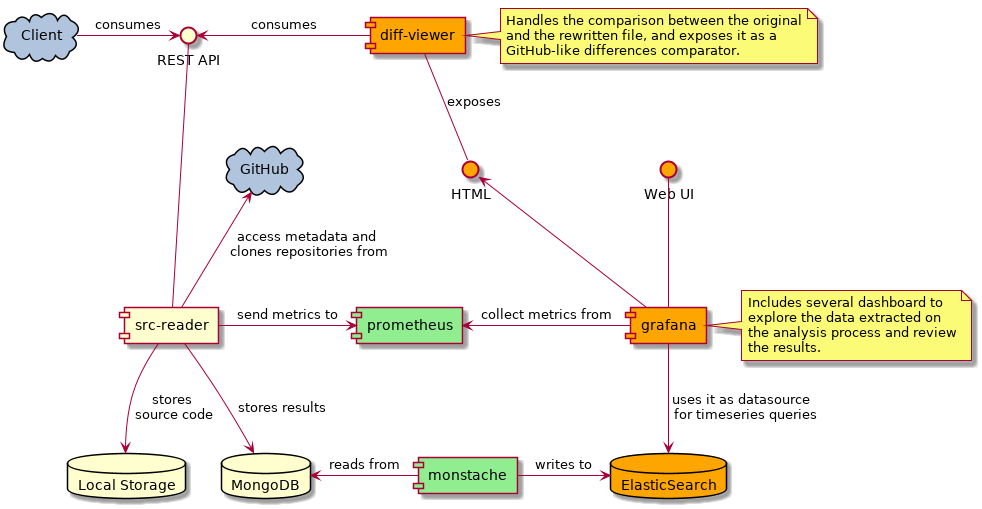
\includegraphics[width=12cm]{implementation/architecture_overview.png}
    \centering
    \caption{Arquitectura general de la Solución}
  \end{figure}


\subsection{Fase: Cálculo}

Tal como se enunció anteriormente, la fase de cálculo consta de diferentes etapas, cada una con un objetivo
bien claro.
Estas etapas se suceden unas a las otras, y la salida de una se utiliza como entrada para la siguiente,
presentando así una cierta secuencialidad estricta.

Para poder dividir y expandir los identificadores que forman parte de una base de código de fuente, 
primero necesitamos analizar los archivos que lo componen y así obtener la información contextual requerida 
por los distintos algoritmos implementados.

Los pasos que se realizan durante esta importación y procesamiento inicial son X:
\begin{enumerate}
  \item \textbf{Acceso al código fuente.} TODO, agregar descripción corta.
  \item \textbf{Parseo.} TODO, agregar descripción corta.
  \item \textbf{Extracción de información requerida.} TODO, agregar descripción corta.
  \item \textbf{Almacenamiento de resultados.} TODO, agregar descripción corta.
\end{enumerate}

\subsection{Acceso al código fuente}

\subsection{Construcción de un AST}
TODO (incluir sección de AST y GO?)
AST en Golang, convenciones de desarrollo, Effective Go, Levesthein distance.

\subsection{Análisis semántico}
Algunos algoritmos, tanto de división como de expansión, requieren de cierta información contextual para poder llevar adelante su tarea.
Por ejemplo, dentro de los algoritmos de división, \textit{Samurai} depende de dos tablas de frecuencia, una de las cuales es específica al programa bajo análisis; y la otra corresponde a un universo mayor de código fuente, independiente del código en cuestión.
Así mismo, el algoritmo de \textit{Expansión Básica} utiliza listas tanto de palabras como frases, extraídas de los comentarios e identificadores asociados a cada una de las funciones analizadas.
En el caso de \textit{AMAP}, para poder efectuar las expansiones, se necesitan establecer tablas de frecuencia por métodos, clases, paquetes e incluso proyectos.

Para poder extraer la información contextual requerida, se realiza un \textbf{análisis semántico} sobre \textit{árbol de sintáxis abstracta (AST)} resultante del paso anterior.

\subsection{Almacenamiento de los resultados}


\subsection{Fase: Visualización}

\subsubsection{Análisis realizados}
\subsubsection{Proyecto Particular}
\subsubsection{Comparación pre/post análisis}
